\documentclass[11pt]{exam}

\makeatletter
\newcommand{\course}[1]{\def\@course{#1}}
\makeatother

\makeatletter
\pagestyle{headandfoot}
\firstpageheader{}{\large \textbf{\@title \ifprintanswers ~-- Solutions \else \fi} \\ \@course}{}
\makeatother


\usepackage{amsmath}
\usepackage{amssymb}
\usepackage{booktabs}
\usepackage{graphicx}
\usepackage{subfig}

\DeclareGraphicsExtensions{.png,.pdf}


\DeclareMathOperator*{\Prob}{P}
\renewcommand{\Pr}{\Prob}
\DeclareMathOperator*{\E}{E}
\DeclareMathOperator*{\var}{var}
\DeclareMathOperator*{\sd}{sd}


\title{Hypothesis Test and Comparison}
\course{STAT-UB.0001 -- Statistics for Business Control}


\begin{document}
\begin{questions}
\fullwidth{\section*{Test on a Population Mean}}

\question (Adapted from Stine and Foster, 4M~16.2).  Does stock in IBM return
a different amount on average than T-Bills?  We will attempt to answer this
question by using a dataset of the 264 monthly returns from IBM between 1990
and 2011.  Over this period, the mean of the monthly IBM returns was $1.26\%$
and the standard deviation was $8.27\%$.  We will take as given that the
expected monthly returns from investing in T-Bills is~$0.3\%$.

\begin{parts}

\part What is the sample?  What are the sample mean and standard deviation?

\begin{solution}
The $n = 264$ monthly IBM returns from 1990 to 2011.  The sample mean and
standard deviation (in \%) are
\begin{align*}
  \bar x &= 1.26 \\
  s &= 8.27
\end{align*}
\end{solution}

\vspace{\stretch{1}}


\part What is the relevant population?  What are the interpretations of
population mean and standard deviation?

\begin{solution}
All monthly IBM returns (past, present, and future).  The population mean,
$\mu$ represents the expected return for a month in the future.  The
population standard deviation, $\sigma$, represents the standard deviation of
the monthly returns for all months (past, present, and future).
\end{solution}

\vspace{\stretch{1}}


\part What are the null and alternative hypotheses for testing whether or not
IBM gives a different expected return from T-Bills (0.3\%)?

\begin{solution}
\begin{align*}
  H_0 &: \mu = 0.3 \\
  H_a &: \mu \neq 0.3
\end{align*}
\end{solution}

\vspace{\stretch{1}}

\newpage

\part Use an appropriate test statistic to summarize the evidence against the
null hypothesis.

\begin{solution}
If the null hypothesis were true ($\mu = 0.3$), then the sample mean would have been a
normal random variable with mean $\mu_{\bar X} = 0.3$ and standard deviation
$\sigma_{\bar X} = \sigma / \sqrt{n}$.  The test statistic
\[
  T = \frac{\bar X - \mu_0}{S/\sqrt{n}}
\]
would follow a $t$ distribution with $n-1=263$ degrees of freedom.  The
observed value of this statistic is
\[
  t = \frac{1.26 - 0.3}{8.27/\sqrt{264}} = 1.886
\]
\end{solution}

\vspace{\stretch{1}}


\part If the null hypothesis were true (there were no difference in expected
monthly returns between IBM and T-Bills) what would be the chance of observing data at
least as extreme as observed?

\begin{solution}
If we approximate the distribution of the test statistic under $H_0$ as a
standard normal random variable, then the chance of observing data at least as
extreme as observed would be
\[
  p = P(|Z| > 1.886) \approx 0.05743.
\]
\end{solution}

\vspace{\stretch{1}}

\part Is there compelling evidence (at significance level 5\%) of a difference
in expected monthly returns between IBM and T-Bills?

\begin{solution}
No, since $p \geq 0.05$, there is not compelling evidence.
\end{solution}

\vspace{\stretch{1}}

\part What assumptions do you need for the test to be valid?  Are these
assumptions plausible?

\begin{solution}
Since $n \geq 30$, we do not need to assume that the population is normal.
We need that the observed sample is a simple random sample from the
population; this might not hold if the period under observation (1990--2011)
is not typical for IBM.
\end{solution}

\vspace{\stretch{1}}

\end{parts}

\newpage

\fullwidth{\section*{Test Statistic and Observed Significance Level ($p$-value)}}

\question \label{ques:tstat} In each of the following examples, for the hypothesis test with
\begin{align*}
  H_0 &: \mu = \mu_0 \\
  H_a &: \mu \neq \mu_0
\end{align*}
find the test statistic ($t$) and the $p$-value.

\begin{parts}

\part $\mu_0 = 5$; $\bar x = 7$; $s = 10$; $n = 36$.

\begin{solution}
\begin{align*}
  t &= \frac{7 - 5}{10/\sqrt{36}} \\
    &= 1.2 \\
  p &\approx P(|Z| > 1.2) \\
    &= 0.2301
\end{align*}
\end{solution}

\vspace{\stretch{1}}


\part $\mu_0 = 90$; $\bar x = 50$; $s = 200$; $n = 64$.

\begin{solution}
\begin{align*}
  t &= \frac{50 - 90}{200/\sqrt{64}} \\
    &= -1.6 \\
  p &\approx P(|Z| > 1.6) \\
    &= 0.1096
\end{align*}
\end{solution}

\vspace{\stretch{1}}

\part $\mu_0 = 50$; $\bar x = 49.4$; $s = 2$; $n = 100$.

\begin{solution}
\begin{align*}
  t &= \frac{49.4 - 50}{2/\sqrt{100}} \\
    &= -3 \\
  p &\approx P(|Z| > 3) \\
    &= 0.002700
\end{align*}
\end{solution}

\vspace{\stretch{1}}


\end{parts}

\question For each example from problem~\ref{ques:tstat}:

\begin{parts}

\part Indicate whether a level 5\% test would reject $H_0$.

\begin{solution}
We reject $H_0$ if $p < 0.05$:
(a) do not reject $H_0$; (b) do not reject $H_0$; (c) reject $H_0$.
\end{solution}

\vspace{\stretch{1}}

\part Indicate whether a level 1\% test would reject $H_0$.

\begin{solution}
We reject $H_0$ if $p < 0.01$:
(a) do not reject $H_0$; (b) do not reject $H_0$; (c) reject $H_0$.
\end{solution}

\vspace{\stretch{1}}

\end{parts}

\newpage
\question Before Facebook's recent redesign, the mean number of ad clicks per
day was 100K.  In the 49 days after the redesign, the mean number of ad clicks
per day was 105K and the standard deviation was 35K.  Is there significant
evidence that the redesign affected the expected number of ad clicks?  Perform
a test at the 5\% level.

\begin{parts}

\part What is the sample?  What is the population?

\begin{solution}
The sample is the number of ad clicks on the measured $n=49$ days.

The population is the number of ad clicks on all days after the redesign.
\end{solution}

\vspace{\stretch{1}}


\part What are the null and alternative hypotheses?

\begin{solution}
Let $\mu$ be the expected clicks per day after the redesign
We use ``thousands of clicks'' as the units for all relevant quantities.

The null hypothesis is that the redesign had no effect on expected ad clicks.
The alternative hypothesis is that $\mu$ changed after the redesign:
\begin{align*}
 H_0 &: \mu = 100 \\
 H_a &: \mu \neq 100
\end{align*}
\end{solution}

\vspace{\stretch{1}}


\part What is the test statistic?

\begin{solution}
The test statistic is based on the sample, the observed clicks in the $n = 49$ days
after the redesign.  Let $\bar x$ denote the mean clicks per day in the
sample; let $s$ denote the sample standard deviation.  Our test statistic is
\begin{align*}
  t &= \frac{\bar x - \mu_0}{s/\sqrt{n}} \\
    &= \frac{105 - 100}{35/\sqrt{49}} \\
    &= 1.
\end{align*}
\end{solution}

\vspace{\stretch{1}}


\part Approximately what is the $p$-value?

\begin{solution}
\begin{align*}
  p &\approx P(|Z| > 1) \\
    &= 0.3137.
\end{align*}
\end{solution}

\vspace{\stretch{1}}


\part What assumptions are you making?

\begin{solution}
We need to assume that the observed sample is a simple random sample from the
population.

Admittedly, the assumption does \emph{not} hold, since there is strong
selection bias in the sample: we are sampling days right after the website
redesign with higher probability than days far into the future.  For example,
we have no chance of sampling a day three years into the future.

Since the assumption does not hold, we are in a bit of an awkward position.
The hypothesis test may not be valid.  One way in which it may not be valid is
the following: it usually takes people a few weeks to adjust to a website
redesign, so the ad click behavior in our sample of 49 days may not be
representative of all future ad click behavior.
\end{solution}

\vspace{\stretch{1}}


\part What is $\alpha$?  What is the result of the test?

\begin{solution}
Despite the caveats mentioned in part (d), we will proceed with the test.
For a level-5\% test, $\alpha = 0.05$.  Since $p \geq  0.05$, we do not reject
$H_0$.  If there were no difference in expected ad clicks before and after the
redesign, there would be a 31.37\% chance of seeing data like we observed.
There is no evidence of a difference.
\end{solution}

\vspace{\stretch{1}}

\end{parts}

\newpage

\fullwidth{\section*{Types of Errors}}

\question In a hypothesis test, our decision will either be ``reject $H_0$''
or ``do not reject $H_0$''.  Under what situations will each of these
decisions be in error?

\begin{solution}
Type I error: $H_0$ is true, but we reject it. \\
Type II error: $H_0$ is false, and we fail to reject it.
\end{solution}

\vspace{\stretch{1}}

\question We reject $H_0$ when the $p$-value is below $\alpha$.  

\begin{parts}

\part If $H_0$ is true, what is the probability of making a Type~I error?

\begin{solution}
We reject $H_0$ when the $p$-value is less than $\alpha$.  This happens when
$|T| > t_{\alpha/2,n-1}$.  So, if the null hypothesis is true, then the
probability of making a Type~I error is
\[
  P(|T| > t_{\alpha/2,n-1}) = \alpha.
\]
\end{solution}

\vspace{\stretch{1}}

\part If $H_0$ is false, what is the probability of \emph{not} making a
Type~II error?

\begin{solution}
We cannot give a direct answer to this question, because it depends on the
true value of $\mu$.  In general, the probability of not making a Type~II
error is called the ``power'' of the test; it is given the symbol $\beta$ or
$\beta(\mu)$.  If $\mu$ is close to $\mu_0$, then $\beta$ will be small (close
to $\alpha$); if $\mu$ is far from $\mu_0$, then $\beta$ will be large (close
to $1$).
\end{solution}

\vspace{\stretch{1}}

\end{parts}

\newpage

\fullwidth{\section*{More $p$-values}}


\question \label{q:pval-tf1} Suppose we perform a hypothesis test and we observe a $p$-value of
$p = .02$.  True or false: There is a 2\% chance that the null hypothesis is
true.

\begin{solution}
False.  The $p$-value is the probability of getting a test statistic at least
as extreme as what was observed.  Heuristically, we can think of this as
\[
  \Pr(\text{Data} \mid \text{$H_0$ is true}) = 2\%.
\]
The statement in the problem is
\[
  \Pr(\text{$H_0$ is true} \mid \text{Data}) = 2\%.
\]
Clearly, this is not the same.
\end{solution}

\vspace{\stretch{1}}


\question \label{q:pval-tf2} Suppose we perform a hypothesis test and we observe a $p$-value of
$p = .02$.  True or false: If we reject the null hypothesis, then there is a 2\%
chance of making a type I error. 

\begin{solution}
False.  We can only make a type I error when the null hypothesis is true.
Thus, the statement in question~\ref{q:pval-tf2} is \emph{exactly the same} as
the statement in question~\ref{q:pval-tf1}.
\end{solution}

\vspace{\stretch{1}}


\question Suppose we perform a hypothesis test and we observe a $T$ test statistic
$t = -2.02$, corresponding to a $p$-value of $p = .02$.  True or false: If we were
to repeat the experiment and the null
hypothesis were actually true, then there would be a 2\% chance of observing a
test statistic at least as extreme as $t = -2.02$.

\begin{solution}
True.  The $p$-value is the probability of getting a test statistic as least
as extreme as the observed value if the null hypothesis were true.
Note: for a one-sided less-than alternative, extreme means ``less than or equal to.''
\end{solution}

\vspace{\stretch{1}}



\newpage


\fullwidth{\section*{Confidence Intervals for Comparing Means}}

\question \label{ques:confint-survey}
Recall the class survey.  Seventeen female and thirty male
students filled out the survey, reporting (among other variables) their
\textsc{gmat} scores and interest levels in the course.  We will use this data
to compare females and males.

\begin{parts}

\part What are the relevant populations?

\begin{solution}
There are two populations: all first-year female Stern MBA students, and all
first-year male Stern MBA students.
\end{solution}

\vspace{\stretch{1}}

\part \label{part:confint-gmat}
For the $14$ female respondents who reported their \textsc{gmat} scores, the
mean was $721$ and the standard deviation was $27$.  For the $28$ male
respondents, the mean was $720$ and
the standard deviation was $39$.  Find a 95\% confidence interval for the
difference in population means.

\begin{solution}

Let sample $1$ be the female \textsc{gmat} scores: $n_1 = 14$, $\bar x_1 = 721$, $s_1 = 27$.
Let sample $2$ be the male \textsc{gmat} scores: $n_2 = 28$, $\bar x_2 = 720$, $s_2 = 39$.  We have
\begin{align*}
  \bar x_1 - \bar x_2 &= 721 - 720 \\
                      &= 1, \\
\mathrm{se}(\bar x_1 - \bar x_2)
  &= \sqrt{\frac{s_1^2}{n_1} + \frac{s_2^2}{n_2}} \\
  &= \sqrt{\frac{(27)^2}{14} + \frac{(39)^2}{28}} \\
  &= 10.
\end{align*}
An approximate 95\% confidence interval for the difference between Stern MBA1 female and
male average \textsc{gmat} scores is
\begin{align*}
  (\bar x_1 - \bar x_2) \pm 2 \mathrm{se}(\bar x_1 - \bar x_2)
    &= 1 \pm (2)(10) \\
    &= 1 \pm 20 \\
    &= (-19, 21).
\end{align*}
(Note: a more precise confidence interval would use $1.96 \mathrm{se}$ instead
of $2 \mathrm{se}$.)
\end{solution}

\vspace{\stretch{1}}



\part \label{part:confint-interest}
For the $17$ female respondents who reported their interest levels in
the course ($1$--$10$), the mean was $5.8$ and the standard deviation was $1.8$.
For the $30$ male respondents, the mean was $6.3$ and the standard deviation
was $2.1$.  Find a 95\% confidence interval for the difference in population
means.

\begin{solution}

Let sample $1$ be the female interest levels: $n_1 = 17$, $\bar x_1 = 5.8$, $s_1 = 1.8$.
Let sample $2$ be the male interest levels: $n_2 = 30$, $\bar x_2 = 6.3$, $s_2 = 2.1$.  We have
\begin{align*}
  \bar x_1 - \bar x_2 &= 5.8 - 6.3 \\
                      &= -0.5, \\
\mathrm{se}(\bar x_1 - \bar x_2)
  &= \sqrt{\frac{s_1^2}{n_1} + \frac{s_2^2}{n_2}} \\
  &= \sqrt{\frac{(1.8)^2}{17} + \frac{(2.1)^2}{30}} \\
  &= 0.3.
\end{align*}
An approximate 95\% confidence interval for the difference between Stern MBA1 female and
male interest levels is
\begin{align*}
  (\bar x_1 - \bar x_2) \pm 2 \mathrm{se}(\bar x_1 - \bar x_2)
    &= (-0.5) \pm (2)(0.3) \\
    &= -0.5 \pm 0.6 \\
    &= (-1.1, 0.1).
\end{align*}
\end{solution}
\vspace{\stretch{1}}

\part For the confidence intervals you constructed in
parts~(\ref{part:confint-gmat}) and~(\ref{part:confint-interest}) to be valid,
what assumptions need to be satisfied?  How could you check these assumptions?

\begin{solution}
We need that the observed samples are simple random samples from the
population.  (We need the samples to be unbiased.)  It is impossible to check
this assumption, but it seems reasonable.

Since the sample sizes are small, we need for the populations to be normal.
We could check this by looking at histograms of the samples.
\end{solution}
\vspace{\stretch{1}}

\end{parts}

\newpage


\fullwidth{\section*{Hypothesis Tests for Comparing Means}}

\question Consider again the class survey data.  We will use the data to
evaluate whether or not there is a significant difference between the female and
the male population means.

\begin{parts}

\part \label{part:pval-gmat}
For the $14$ female respondents who reported their \textsc{gmat} scores,
the mean was $721$ and the standard deviation was $27$.  For the $28$ male
respondents, the mean was $720$ and the standard deviation was $39$.  If the
population means were equal what would be the chance of seeing a difference in
sample means as large as observed?

\begin{solution}
To answer this, we first compute a test statistic:
\begin{align*}
  t &= \frac{\bar x_1 - \bar x_2}{\mathrm{se}(\bar x_1 - \bar x_2)} \\
    &= \frac{1}{10} \\
    &= 0.1.
\end{align*}
If the population means were equal, then the test statistic would be 
approximately normally distributed; the chance of seeing a difference in sample
means as large as observed would be
\begin{align*}
  p &\approx P(|Z| \geq 0.1) \\
    &\approx 0.9203.
\end{align*}
That is, it would be very typical to see such a difference.
\end{solution}
\vspace{\stretch{1}}


\part \label{part:pval-interest}
For the $27$ female respondents who reported their interest levels in
the course ($1$--$10$), the mean was $5.8$ and the standard deviation was $1.8$.
For the $30$ male respondents, the mean was $6.3$ and the standard deviation
was $2.1$.  If the population means were equal what would be the chance of
seeing a difference in sample means as large as observed?

\begin{solution}
This is similar to the previous problem:
\begin{align*}
 t &= \frac{\bar x_1 - \bar x_2}{\mathrm{se}(\bar x_1 - \bar x_2)} \\
   &= \frac{-0.5}{0.3} \\
   &= -1.7 \\
 p &\approx P(|Z| \geq 1.7) \\
   &\approx 0.08913.
\end{align*}
It would be very typical to see a difference in sample means as large as
observed.
\end{solution}
\vspace{\stretch{1}}

\part What is the relationship between the confidence intervals
in Question~\ref{ques:confint-survey} and your answers to
parts~(\ref{part:pval-gmat}) and~(\ref{part:pval-interest})?

\begin{solution}
When the 95\% confidence intervals contain $0$, the $p$-values for testing for
a difference are greater than $0.05$ (the differences are not significant at
level 5\%).
\end{solution}
\vspace{\stretch{1}}

\end{parts}


\newpage

\fullwidth{\section*{Case Study: Bicycle Passing Distance}}



\question Here are boxplots of the passing distances (in meters) for a bike
rider with and without a helmet.  Is there evidence that the passing distance
differs when the rider has a helmet?
\begin{center}
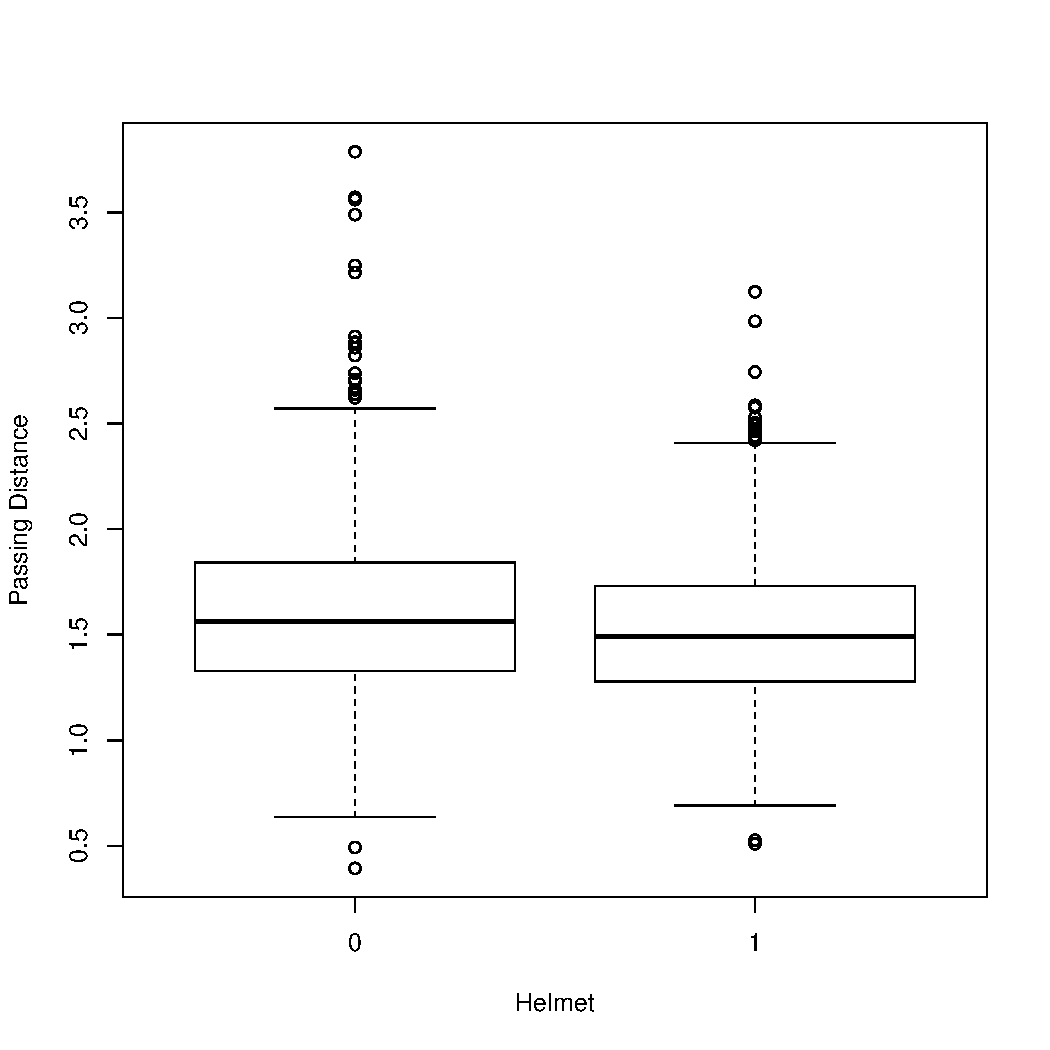
\includegraphics[width=0.5\textwidth]{passing-by-helmet}
\end{center}
Here are the sample statistics for the passing distance without a helmet:
$n_1 = 1206$, $\bar x_1 = 1.61$, $s_1 = 0.405$.  Here are the sample
Here are the sample statistics for the passing distance with a helmet:
$n_2 = 1149$, $\bar x_2 = 1.52$, $s_2 = 0.354$.

Formulate the problem as a hypothesis test, using significance level 5\%.

\begin{parts}

\part What are the populations?

\begin{solution}
Population 1: all passing distances while not wearing a helmet.

Population 2: all passing distances while wearing a helmet.
\end{solution}
\vspace{\stretch{1}}

\part What are the null and alternative hypotheses?

\begin{solution}
\begin{align*}
  H_0 &: \mu_1 = \mu_2 \quad\text{(same mean distance for both populations)} \\
  H_a &: \mu_1 \neq \mu_2.
\end{align*}
\end{solution}
\vspace{\stretch{1}}

\part What are the samples?

\begin{solution}
All recorded passing distances, without and with a helmet.
\end{solution}
\vspace{\stretch{1}}

\newpage

\part What is the test statistic?

\begin{solution}
\begin{align*}
  \bar x_1 - \bar x_2
    &= 1.61 - 1.52 \\
    & = 0.09 \\
  \mathrm{se}(\bar x_1 - \bar x_2) 
    &= \sqrt{\frac{(0.405)^2}{1206} + \frac{(0.354)^2}{1149}} \\
    &= 0.016 \\
  z &= \frac{\bar x_1 - \bar x_2}{\mathrm{se}(\bar x_1 - \bar x_2)} \\
    &= \frac{0.09}{0.016} \\
    &= 5.6
\end{align*}
\end{solution}
\vspace{\stretch{1}}

\part Approximately what is the $p$-value and the result of the test?

\begin{solution}
\begin{align*}
  p &\approx P(|Z| \geq 5.6) \\
    &< 5.733 \times 10^{-7}.
\end{align*}
If there were no difference in average passing distance with and without a
helmet, then there would be less than a $5.733\times 10^{-5}$ chance of seeing
data like that observed.  There is substantial evidence of a difference;  we
reject $H_0$.
\end{solution}
\vspace{\stretch{1}}


\part Find a 95\% confidence interval for the difference in passing
difference with and without a helmet.

\begin{solution}
\[
  0.09 \pm 2 (0.016)
\]
With 95\% confidence, the difference in population means is between 0.058 and
0.122 meters.
\end{solution}

\vspace{\stretch{1}}


\end{parts}




\end{questions}


\end{document}
